\subsection{Pacman (by Heithoff)}
In the following the model for the Pacman controller is presented. The goal is to collect as many biscuits and coins as possible and to avoid the ghosts. After introducing the interface which is used here two controllers for Pacman are shown. There is a simple controller which was used in the early stages of the IDE integration to test everything and then a more complex controller that can actually survive a few levels.

\subsubsection{Interface}
\begin{figure}[t!]
	\caption{Visualization of the Pacman wrapper}
	\label{fig:visPacmanWrapper}
	\centering
	\includegraphics[scale=0.7]{pictures/VisualizationPacmanWrapper.png}

\begin{lstlisting}[label=lst:pacmanWrapper, caption=Interface of the Pacman Wrapper, language=EMAM]
ports 
	in (0cm: 180cm) ghostX[4],
	in (0cm: 210cm) ghostY[4],
	in (0 : 1 : 3) ghostDirection[4],
	in B ghostEatable[4],
	in B ghostEaten[4],
	in (0cm: 180cm) pacManX,
	in (0cm: 210cm) pacManY,
	in B pacManEaten,
	in (0:oo) pacManLives,
	in (0:oo) pacManScore,
	in Z^{22,19} map,
	out (0 : 1 : 3) newPacmanDirection;
\end{lstlisting}
\end{figure}
The project's main component is PacmanWrapper. The main task of the wrapper is to provide a shared interface. Listing \ref{lst:pacmanWrapper} shows the input and output ports. As for the inputs, the ghosts' and the Pacman's position are given, the direction the ghosts are facing, information about the ghosts' vulnerability, as well as the current map. The only output port is the new direction the Pacman should walk. \newline
The wrapper also holds the current controller. This way the controller is easily exchangeable without changing any of the code needed for the ide. All input ports of the wrapper are connected to the corresponding ports of the controller and the output port of the controller is also connected to the output port of the wrapper. \newline
To connect the web assembly of the main component with the Pacman emulator a new JavaScript file was created. Its main functionalities is to extract the needed informations out of the emulator, pass it to the web assembly, execute it and then give the output back to the emulator. In order to be able to extract needed information out of the emulator some modifications were needed. In its original state the emulator did not offer access to the current game object, thus the \textit{Pacman} class was extended by these functions. Due to the fact Pacman is a playable game, its input is given as a key-press-event in JavaScript. So the output of the web assembly, which is a number from 0 to 3, is mapped to a corresponding key-press-event which then gets triggered. The emulator is running with 30 frames per second, which also leads to 30 iterations of the game per second. Because the emulator is running asynchronously the component is executed at a double of that rate in order to track every position change.

\subsubsection{C\&C modeling - Pacman (simple)}
\begin{figure}
	\caption{Visualization of the Pacman controller (simple)}
	\label{fig:visPacmanSimple}
	\centering
	\includegraphics[width=\textwidth]{pictures/VisualizationPacmanSimple.png}
\end{figure}
In figure \ref{fig:visPacmanSimple} the design of a simple controller is shown. It has four subcomponents:
\begin{itemize}
	\item nearestGhost: Is given the x - and y - position of every ghost and the x - and y - position of the Pacman. It then iterates over all ghosts and calculates the nearest ghost and gives back its index.
	\item picker: Is given all ghost informations as input as well as an index and gives back the ghost information of the ghost at this index.
	\item away: Is given one ghost's informations as well as Pacman's and calculates a new direction for the Pacman facing away from the ghost. The output is one of the four possible directions mapped from the numbers 0 to 3.
	\item tryDir: Gets as input the position of Pacman, the current map as well as a direction the Pacman should try to walk. If there is no wall blocking the way the initial direction is outputted. On the other hand, if there is a wall blocking the way it tries to walk orthogonally left or up. If it fails it will walk right or down respectively.
\end{itemize}
The controller connects the subcomponents in the shown order: It calculates the nearest ghost, passes its index to the picker which then again passes the corresponding ghost to the \textit{away} component. This calculates the direction facing away from said ghost and the \textit{tryDir} component then avoids running into walls. This leads to a controller that runs away from the ghosts with some success but it is only determined by the nearest ghost and has no other goals. Due to the fact that \textit{tryDir} always tries to walk to the left (or top) first, this can lead to some stuttering as soon as the Pacman walked enough to the right that there is again space to the left. \newline
This design is very simple and not very successful. It shows the concept of C\&C modeling in its basics and is therefore listed here. The next controller is a lot more complex and can easily beat up to 10 levels.

\subsubsection{C\&C modeling - Pacman (complex)}
\begin{figure}
	\caption{Visualization of the Pacman controller (complex)}
	\label{fig:visPacman20}
	\centering
	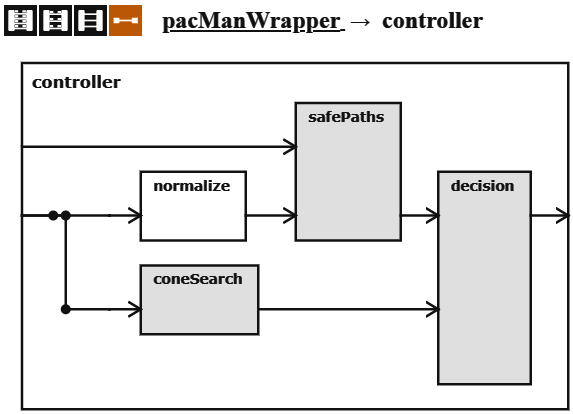
\includegraphics[width=\textwidth]{pictures/Pacman/Controller20.png}
\end{figure}

The more complex Pacman controller is shown in figure \ref{fig:visPacman20}.
It has three main subcomponents:
\begin{itemize}
	\item \textit{safePaths}: This component is responsible for checking all the paths leading from Pacman into the labyrinth for safety. This is done by searching in each of the four possible directions until a wall or intersection is found.	
	\item \textit{coneSearch}: Searches in cones in each of the four directions for enemies and coins and gives back a score for each direction.	
	\item \textit{decision}: The decision component evaluates all data from the other two components. Based on those values it decides which direction the Pacman should go next.	
\end{itemize}
The last component \textit{normalize} not listed here is only responsible for increasing all position values from the ghosts and Pacman by 1 to fit the indexation from the math library.
We will now go into detail for the three main component.
\newline

\emph{Safe Paths} \newline
\begin{figure}
	\caption{Visualization of Safe Paths}
	\label{fig:safePaths}
	\centering
	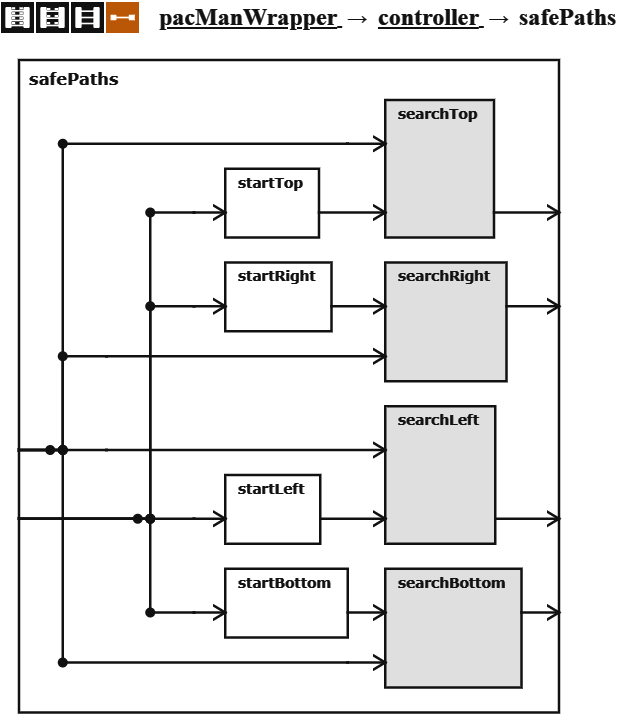
\includegraphics[scale=0.75]{pictures/Pacman/safePaths.png}
\end{figure}
In figure \ref{fig:safePaths} the \textit{safePaths} component is shown. It contains a subcomponent for each direction and some starting values. It gives back whether the four directions are safe or not. A direction is safe if there is a wall blocking it (no path) or there is no enemy on its path until the next intersection. This is calculated by ``going'' the path. This could be done with a single component looping through the path to the next intersection. Due to the fact that this would contradict the conditions on C\&C components stated before it is split up into subcomponents. Each path in this labyrinth has a length of at most 10. So the task is divided into 10 components as one can partially see in fig. \ref{fig:search}. Each of those checks whether the current position is safe and then calculate the position to check for the next component. This way the runtime is fixed and the code is better parallelizable.
\begin{figure}
	\caption{Visualization of one Search}
	\label{fig:search}
	\centering
	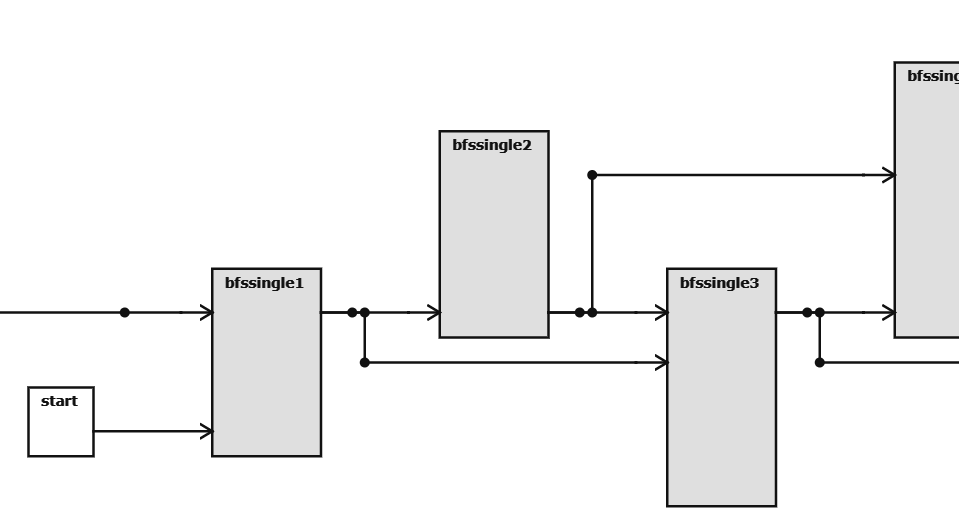
\includegraphics[width=\textwidth]{pictures/Pacman/Search.png}
\end{figure}

\begin{figure}
	\caption{Visualization of one Single Search Component}
	\label{fig:searchSingle}
	\centering
	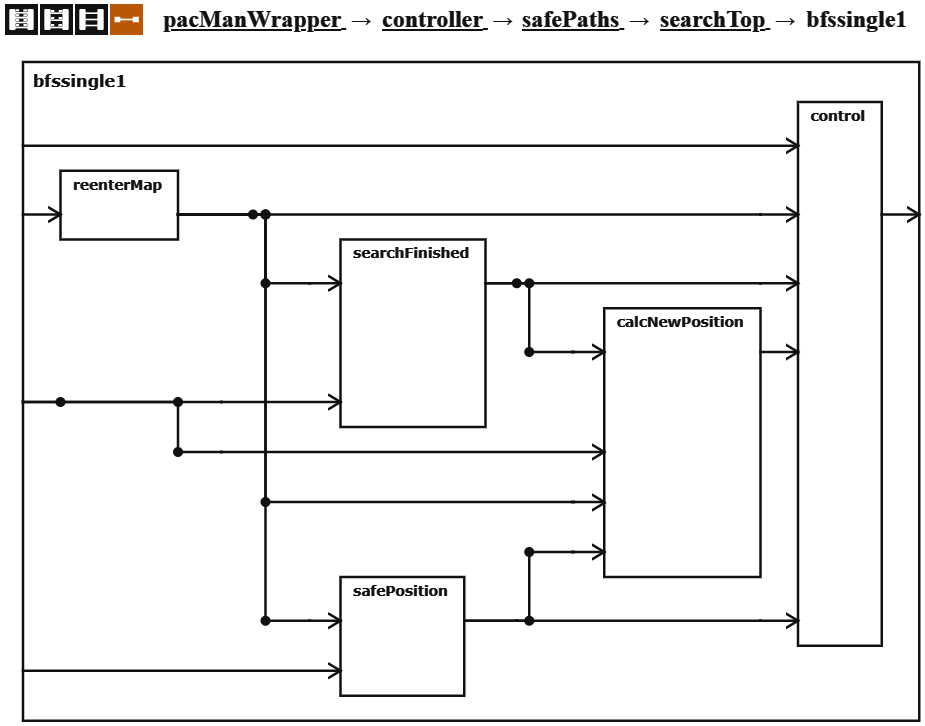
\includegraphics[width=\textwidth]{pictures/Pacman/SearchSingle.png}
\end{figure}
The task of one of the 10 subcomponents is again split up into 5 subtasks (see fig. \ref{fig:searchSingle}):
\begin{itemize}
	\item \textit{reenterMap}: If the previous component calculated a position outside of the map (e.g. leaving the map on the right through the tunnel), reenter the map on the other side.
	\item \textit{safeFinished}: The search is finished if it is marked as finished by a previous search component or a wall is found (only when there is no path).
	\item \textit{safePosition}: Loops through the four ghosts and check whether their position matches the current position. If an unsafe tile is found, the search is marked as finished and not safe.
	\item \textit{calcNewPosition}: Looks for free ways in the adjacent tiles. If there are more than two free tiles (no wall), an intersection is reached and the search can be marked finished. Otherwise this component gives back the next position which is different from the previous one.
	\item \textit{control}: The control unit evaluates all data from the other components and gives back a corresponding new position and whether the search until now is safe or not.
\end{itemize}

\emph{Cone Search} \newline
\begin{figure}
	\caption{Visualization of Cone Search}
	\label{fig:cone}
	\centering
	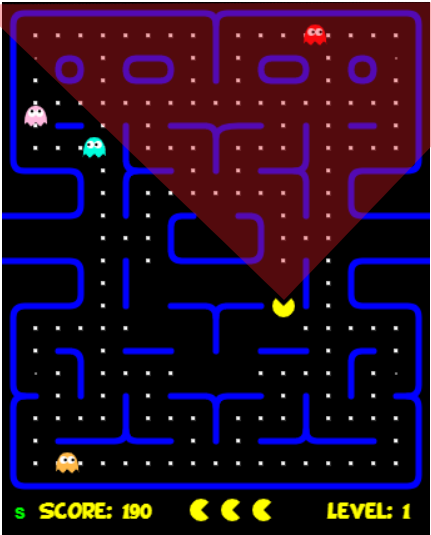
\includegraphics[width=\textwidth]{pictures/Pacman/Cone.png}
\end{figure}
The \textit{ConeSearch} component searches through the map in cones (see figure \ref{fig:cone}). This way each direction can be given a value which increases when biscuits and coins are found and decreases when ghosts are found. The following weights are used in the most current version:
\begin{itemize}
	\item biscuit: 50
	\item coin: 200
	\item enemy (facing towards Pacman): -10
	\item enemy (facing a different direction): -4
	\item enemy (eatable): 1000
\end{itemize}
The values shrink with the distance to Pacman. The biscuit/coin value shrink squared and the enemy value linear with the distance. This way near objectives are valued more and Pacman does not go for only far away biscuits/coins if there already are nearby ones. But if all biscuit/coin values are small the maximum gets increased by a fix amount, so Pacman goes for far away biscuits/coins if there are no around. In the end for each direction a value is returned by combining the biscuits/coins value and the enemy value. 
\begin{figure}
	\caption{Visualization of Cone Search}
	\label{fig:coneSearch}
	\centering
	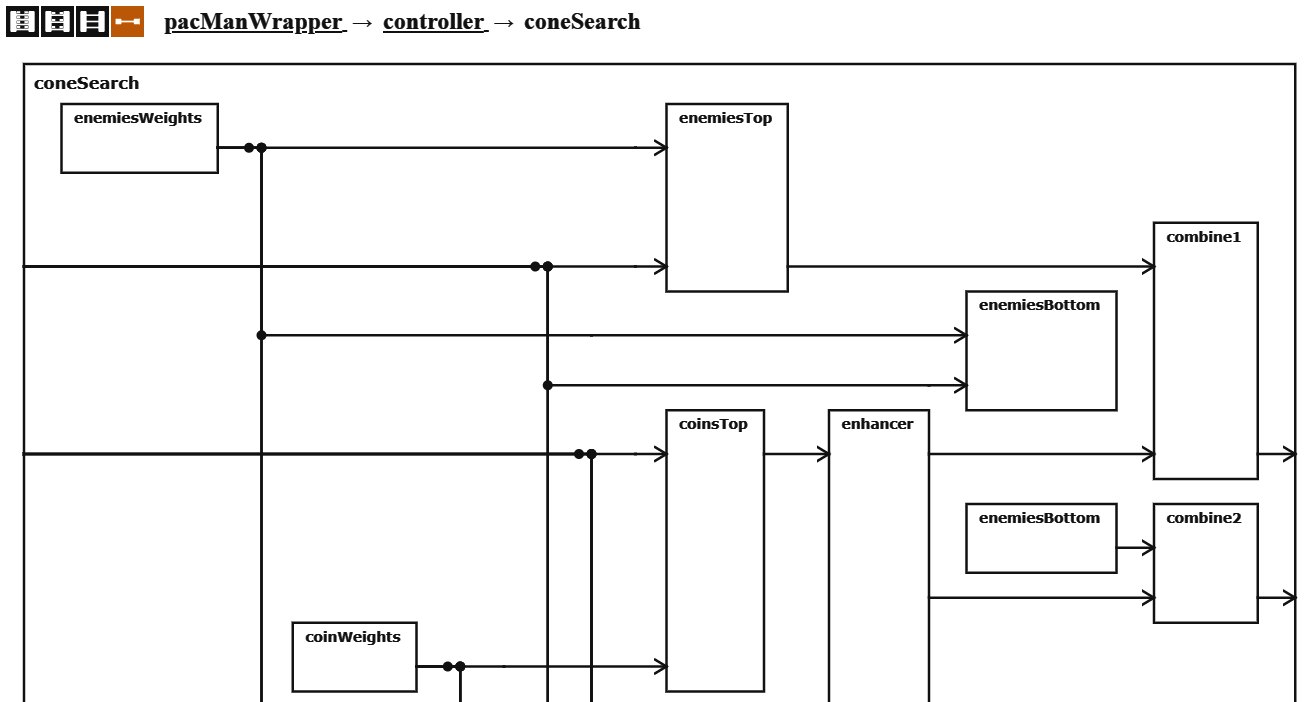
\includegraphics[width=\textwidth]{pictures/Pacman/ConeSearch.png}
\end{figure}

In the visualization of the component (see fig. \ref{fig:coneSearch}) one can see the different kind of subcomponents:
\begin{itemize}
	\item \textit{enemiesWeights} and \textit{coinWeights}: some constants for weighting biscuits, coins and ghost values. This design allows easy adjustments.
	\item \textit{enemies(Top)}: searches for enemies in the (top) cone and gives back its value.
	\item \textit{coins(Top)}: searches for biscuits/coins in the (top) cone and gives back its value.
	\item \textit{enhancer}: increases the maximum biscuits/coins value if it is small.
	\item \textit{combine}: combines the values for biscuits/coins and enemies for a direction.
\end{itemize}

\emph{Decision} \newline
\begin{figure}
	\caption{Visualization of Cone Search}
	\label{fig:decision}
	\centering
	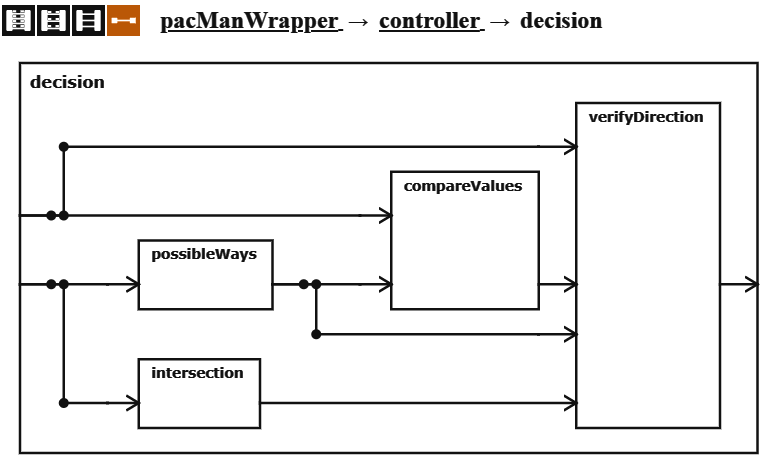
\includegraphics[width=\textwidth]{pictures/Pacman/Decision.png}
\end{figure}
The \textit{decision} component gets all data from \textit{safePaths} and \textit{coneSearch} and makes a final decision on where to go. Beside the maximum value for a direction and whether it is safe or not, the decision is based on a few additional information. E.g. the top direction has the maximum value from the cone searches but it is blocked by a wall or not safe. Then another direction has to be chosen. Here an orthogonal direction (left or right) is preferred to stay near to the desired one (top). In addition, to prevent stuttering a new path is only chosen if the current one is not safe anymore or an intersection is reached.
In fig. \ref{fig:decision} one can see the four subcomponents of \textit{safePaths}:
\begin{itemize}
	\item \textit{intersection}: Gives back whether Pacman is located on a tile with more than 2 Paths leading from it.
	\item \textit{possibleWays}: Gives back which directions are not blocked by a wall.
	\item \textit{compareValues}: Calculates the safe direction with the maximum value. If this direction is blocked, a new direction has to be chosen.
	\item \textit{verifyDirection}: Checks whether the chosen direction is opposing the previous one. This is only allowed if the previous direction is not safe anymore or an intersection is reached.
\end{itemize}